\section{Introduction}

Операции в непосредственной близости от небольших тел чрезвычайно сложны из-за их неопределенной динамической среды. 
Автономное наведение и навигация вокруг небольших тел требуют быстрого и точного моделирования гравитационного поля для потенциальных бортовых вычислений.
В этой статье исследуется основанный на моделях машинного обучения подход к вычислению и прогнозированию гравитационного ускорения вокруг малых тел неправильной формы.
В частности, используется теория машин экстремального обучения (ELM).

Миссия NASA OSIRIS REx по возврату образцов астероидов находилась в непосредственной близости от астероида Бенну в августе 2018 года и вскоре после сближения с космическим кораблем запустила карту Feedforward Networks, способную изучать взаимосвязь между положением космического корабля и гравитационным ускорением.
На основе полученных данных происходит моделирование гравитационного поля методами основанными на физических походах.
Нейронные сети на основе ELM обучаются без итеративной настройки, что значительно сокращает время обучения.
Анализ характеристик моделей постоянной плотности для астероида 25143 Итокава и кометы 67/P Чурюмов-Герасименко показывает, что SLFN на основе ELM способны изучать желаемые функциональные взаимосвязи как глобально, так и в выбранных локализованных областях вблизи поверхности.

Последнее приводит к созданию надежного нейронного алгоритма для бортового расчета в реальном времени гравитационного поля, необходимого для наведения и управления в операциях в непосредственной близости от поверхности астероида.

\section{References Review}

Основным источником информации является ~\cite{FURFARO2021617}, обзором которой является данная глава. Тут описаны физические подходы для исследования и модели машинного обучения.


\section{Main Part}

За последние несколько лет появился большой интерес к отправке космических аппаратов-роботов к небольшим телам в Солнечной системе, включая кометы (например, миссия Rosetta) и околоземные астероиды (NEAs, например, миссия Хаябуса).

Любая из текущих и предстоящих миссий по астероидам или кометам требует планирования ряда надежных операций в непосредственной близости от небольших тел.
Такие операции, как правило, являются чрезвычайно сложными и усложняются рядом факторов, включая неправильную форму и распределение массы, слабое и неопределенное гравитационное поле, ускорения из-за дегазации комет, а также возмущающие ускорения из-за солнечного излучения, которые во многих случаях имеют тенденцию быть того же порядка, что величины ускорения свободного падения.
Из-за этих факторов орбитальная динамика вокруг малых тел значительно отклоняется от идеального кеплеровского движения и имеет тенденцию быть очень нерегулярной.
Для автономных операций с обратной связью может потребоваться эффективное и быстрое представление гравитационного поля вблизи поверхности для бортовых расчетов управляющей команды ускорения и / или синхронизации импульса.

Классический подход к моделированию гравитационного поля основан на методе разложения по сферическим гармоникам. Многополюсное расширение в основном использовалось для представления поля гравитационного потенциала из-за высокой точности, обеспечиваемой относительно низкими вычислительными затратами.
\[
    U(r,\phi,\theta) = \frac{GM}{r}
        \sum_{n = 0}^{\infty} \left( \frac{R^*}{r}\right)
        \sum_{m = 0}^{m} P_{nm}\sin\phi \cdot (a_{nm}\cos(m\theta) + b_{nm}\sin(m\theta)),
\]
где $a_{nm}, \quad b_{nm}$ - коэффициенты сферических гармоник, $R^*$~-~усредненный радиус поверхности тела, $P_{nm}$ - полином Лежандра.

Действительно, после измерения гравитационных коэффициентов (например, с помощью орбитальной кампании радиотехники на этапе эксплуатации) гравитационное ускорение можно легко вычислить, взяв пространственные производные потенциальных гармоник с желаемой степенью точности.
\begin{figure}[h]
    \centering
    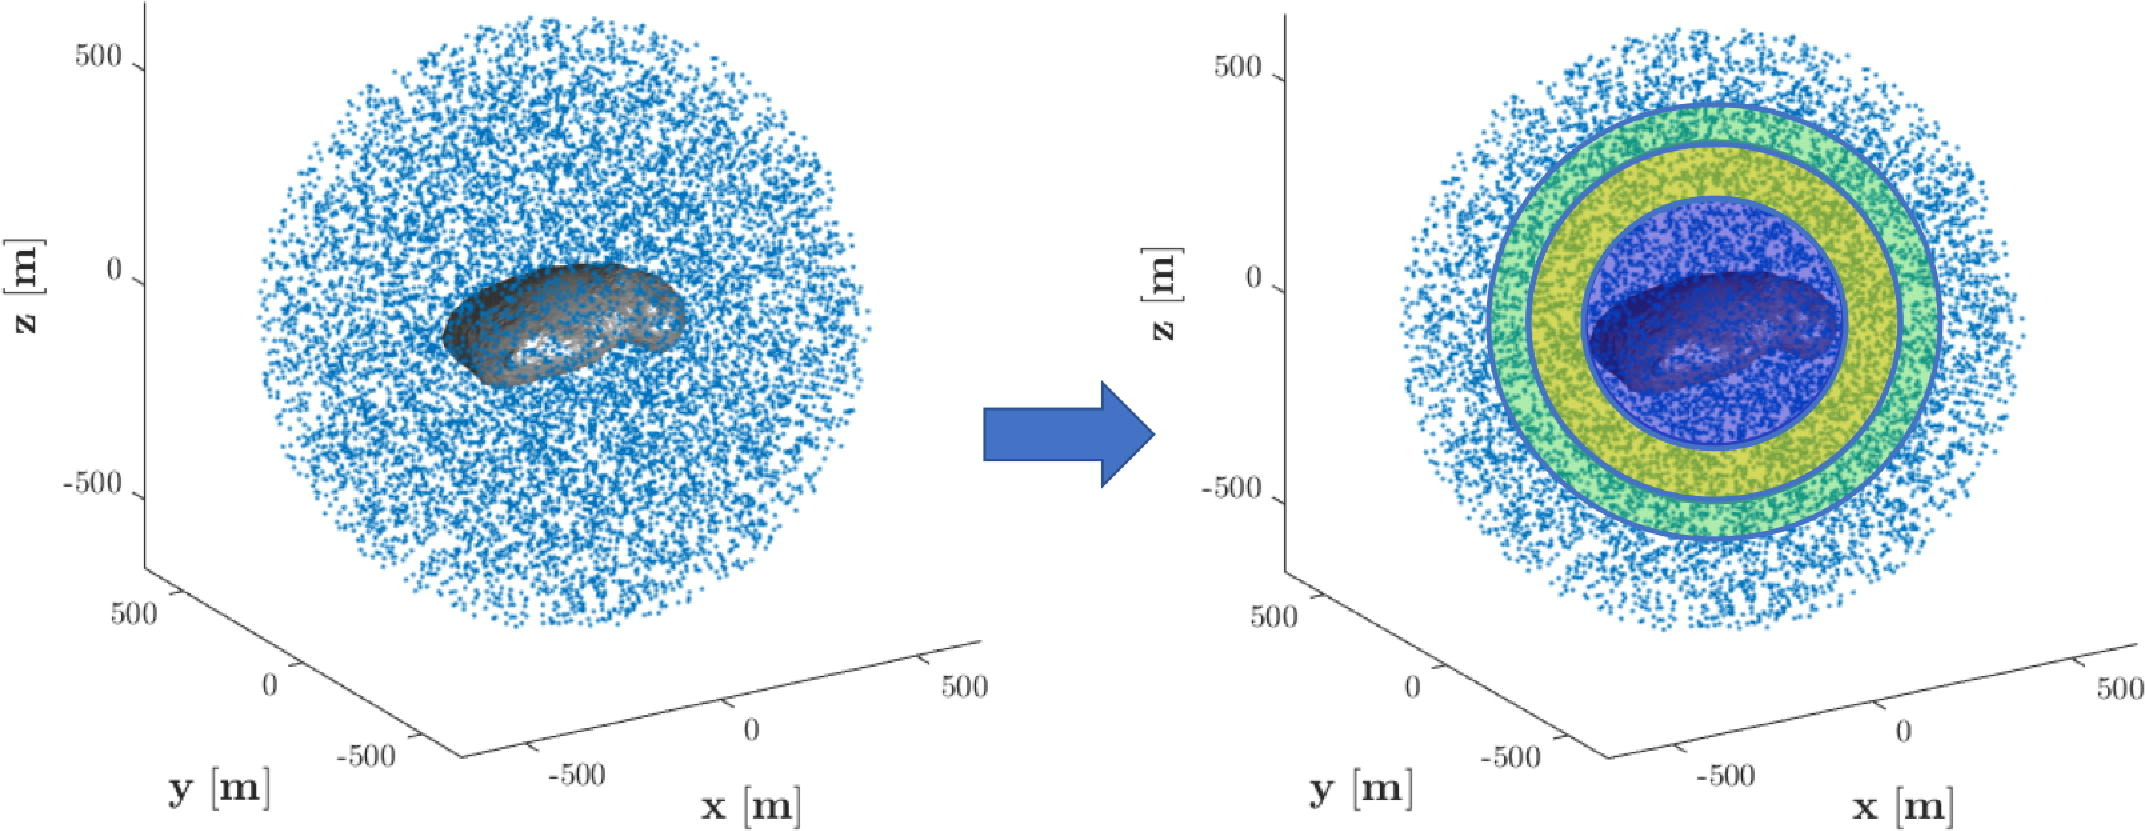
\includegraphics[width=0.8\textwidth]{chapters/tikhonov_s2/images/train_1}
\end{figure}
Однако математическая сходимость ряда гарантируется только для точек за пределами так называемой сферы Бриллюэна, т. Е. Сферы с центром в центре расширения и описывающей внешний элемент массы малого тела (Russell and Arora, 2012a).
Известно, что внутри сферы расходятся серии гармоник.

В то время как расхождение не представляет проблемы для малых тел, близких к сферическим, оно вызывает серьезные проблемы для тел неправильной формы и распределения массы. В результате внешний потенциал не может моделировать гравитационное поле внутри сферы Бриллюэна. Существуют альтернативы потенциальной модели внешней гравитации, например модель массовой концентрации (mascon) (Werner, Scheeres, 1996a) и модель полиэдра (Takahashi et al., 2013a).

В то время как первая модель имеет тенденцию быть неточной, модель многогранников может точно описывать гравитационное поле как функцию плотности (однородной или неоднородной).
\[
    \nabla U(\mathbf{r}) = \sigma G
    \left(
        - \sum_{e \in \text{edges}}\mathbf{E}_e \mathbf{r}_e L_e
        + \sum_{f \in \text{faces}}\mathbf{F}_f \mathbf{r}_f \omega_f
    \right),
\]
где $\sigma$ - средняя плотность, $\mathbf{E}_e, \mathbf{F}_f$ - матрицы и $L_e, \omega_f$ - скаляры сформулированные в Werner and Scheeres (1996b).
\begin{figure}[h]
    \centering
    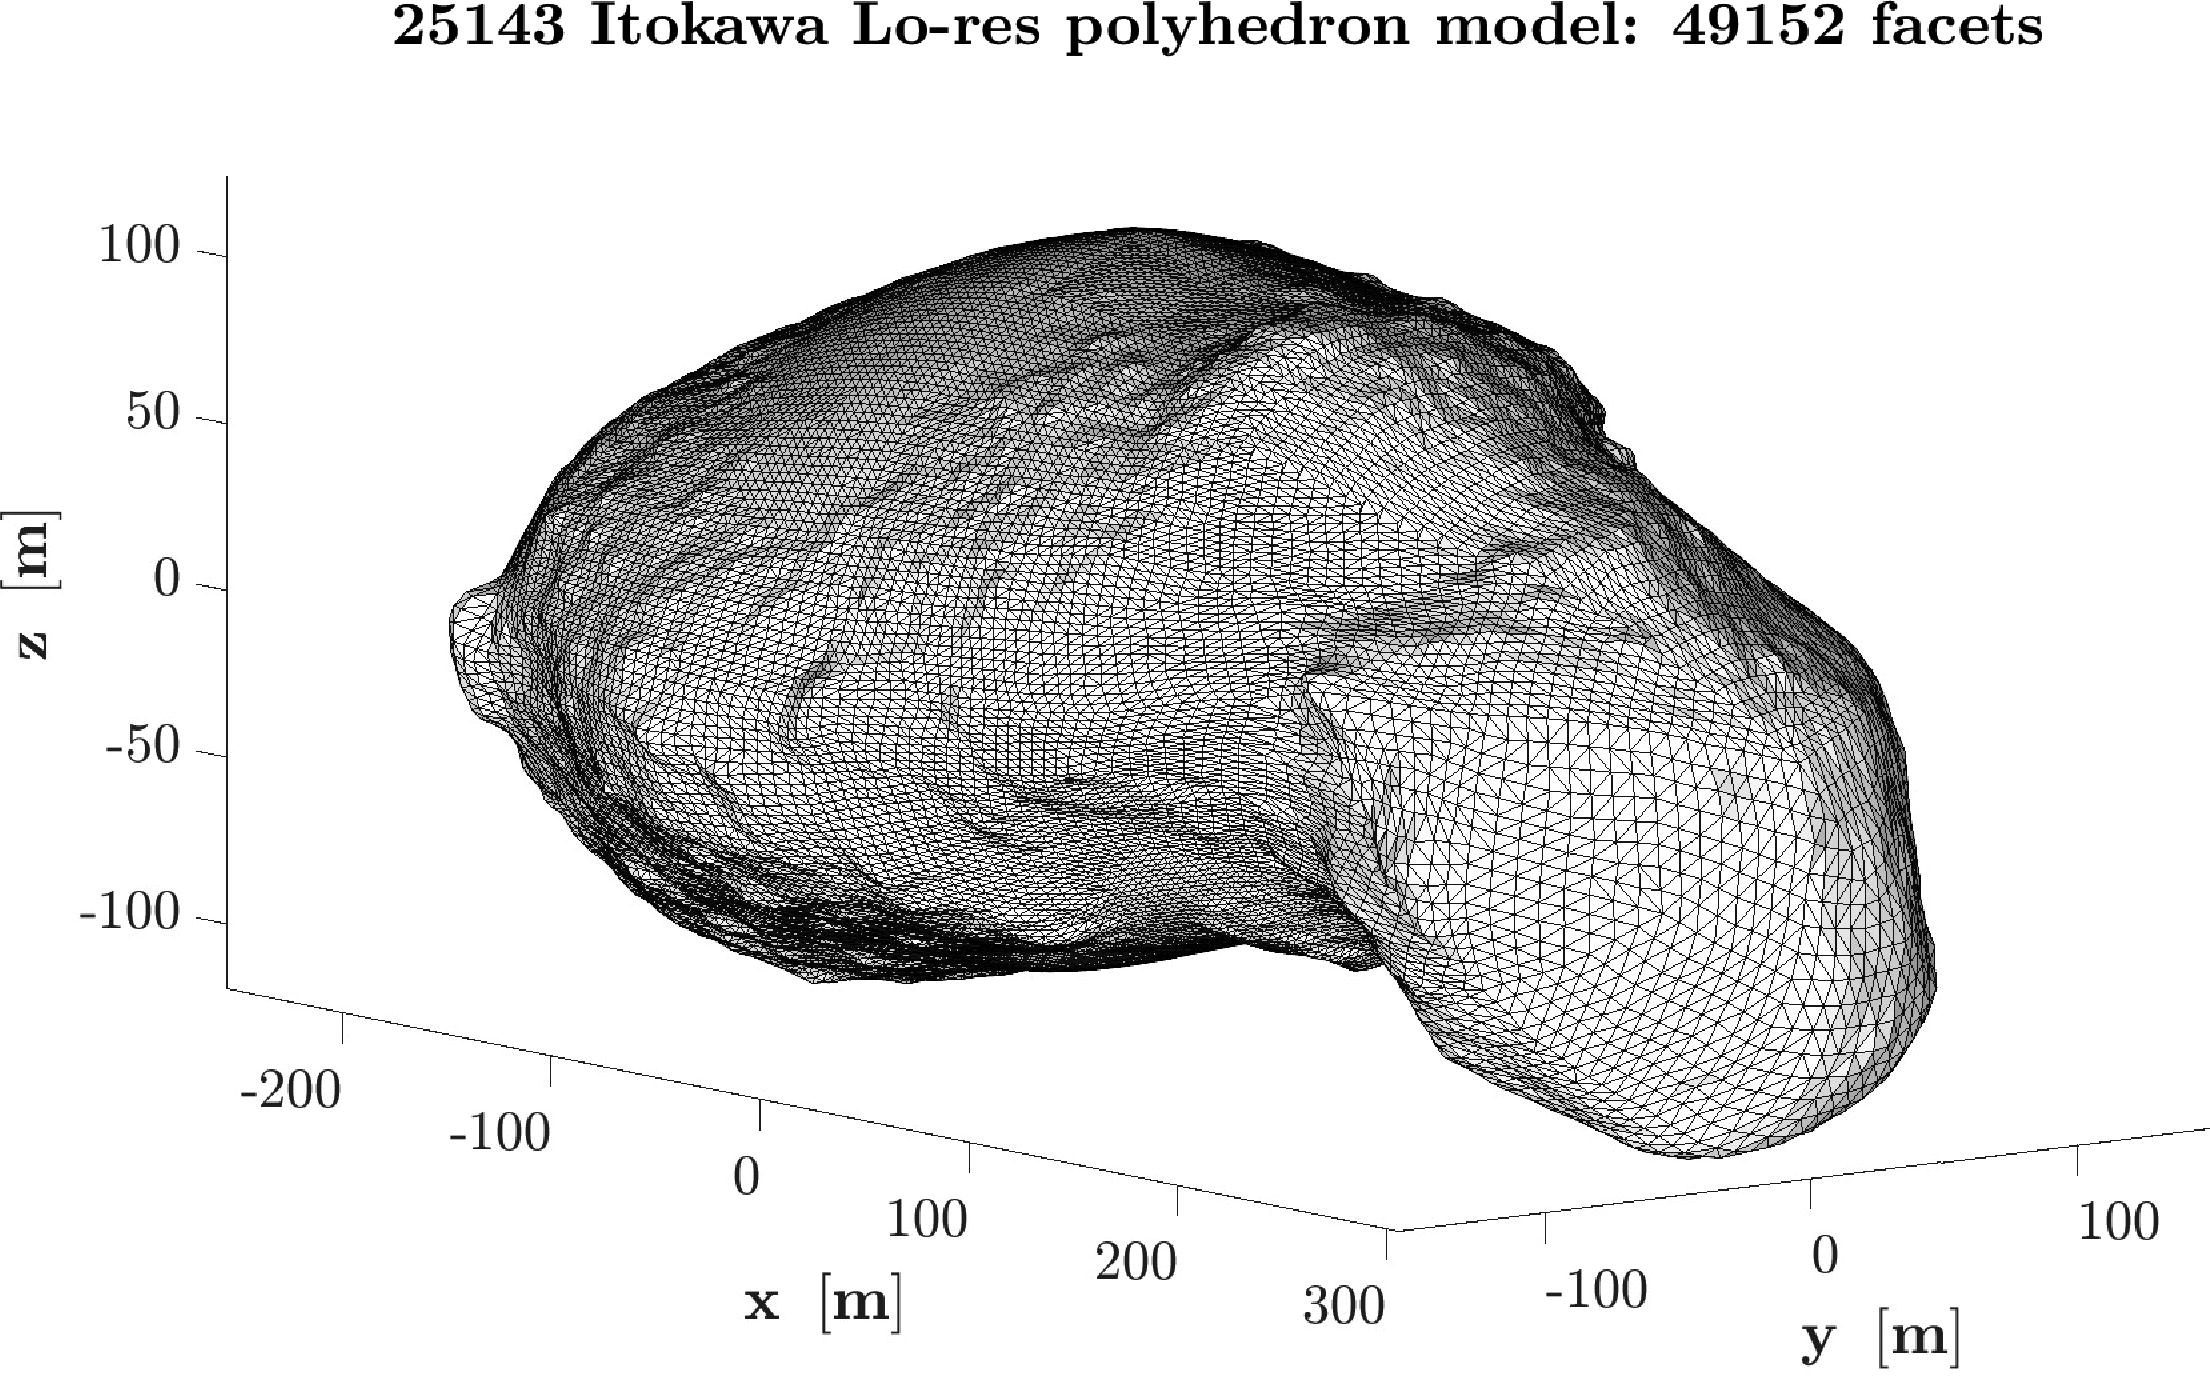
\includegraphics[width=0.8\textwidth]{chapters/tikhonov_s2/images/poly}
    \label{fg:1}
\end{figure}

Однако она требует больших вычислительных ресурсов и, как правило, не подходит для наземного моделирования методом Монте-Карло или для расчета динамики космического корабля на борту.

В последнее время проявился интерес к изучению новых методов моделирования гравитационного поля с использованием подхода, основанного на данных.
Общая идея состоит в том, чтобы напрямую аппроксимировать карту между положением вокруг астероида и соответствующим гравитационным ускорением, используя парадигму обучения, основанную на статистическом машинном обучении.

В этой главе предлагается методология моделирования гравитационного поля неправильного небольшого тела для быстрого, точного и эффективного расчета гравитационного ускорения как функции относительного положения вокруг небольшого исследуемого тела.
Методология основана на недавно разработанном подходе машинного обучения под названием Extreme Learning Machines (ELM), который использует однослойную сеть прямого распространения (SLFN) для моделирования нелинейных отношений между входами и выходами.
\begin{itemize}
\item Модель нейронной сети:
\[
    \mathbf{y}_j = \sum_{i=1}^L \mathbf{\beta}_i
        h_i(\mathbf{x}_j,\mathbf{\omega}_i,{b}_i),
\]
где $\mathbf{\beta}_i,\mathbf{\omega}_i,{b}_i$ - веса модели, $\mathbf{x}_j$ - входные данные, $\mathbf{y}_j$ - выходные данные, $h$ - функция активации.
\end{itemize}
\begin{figure}[h]
    \centering
    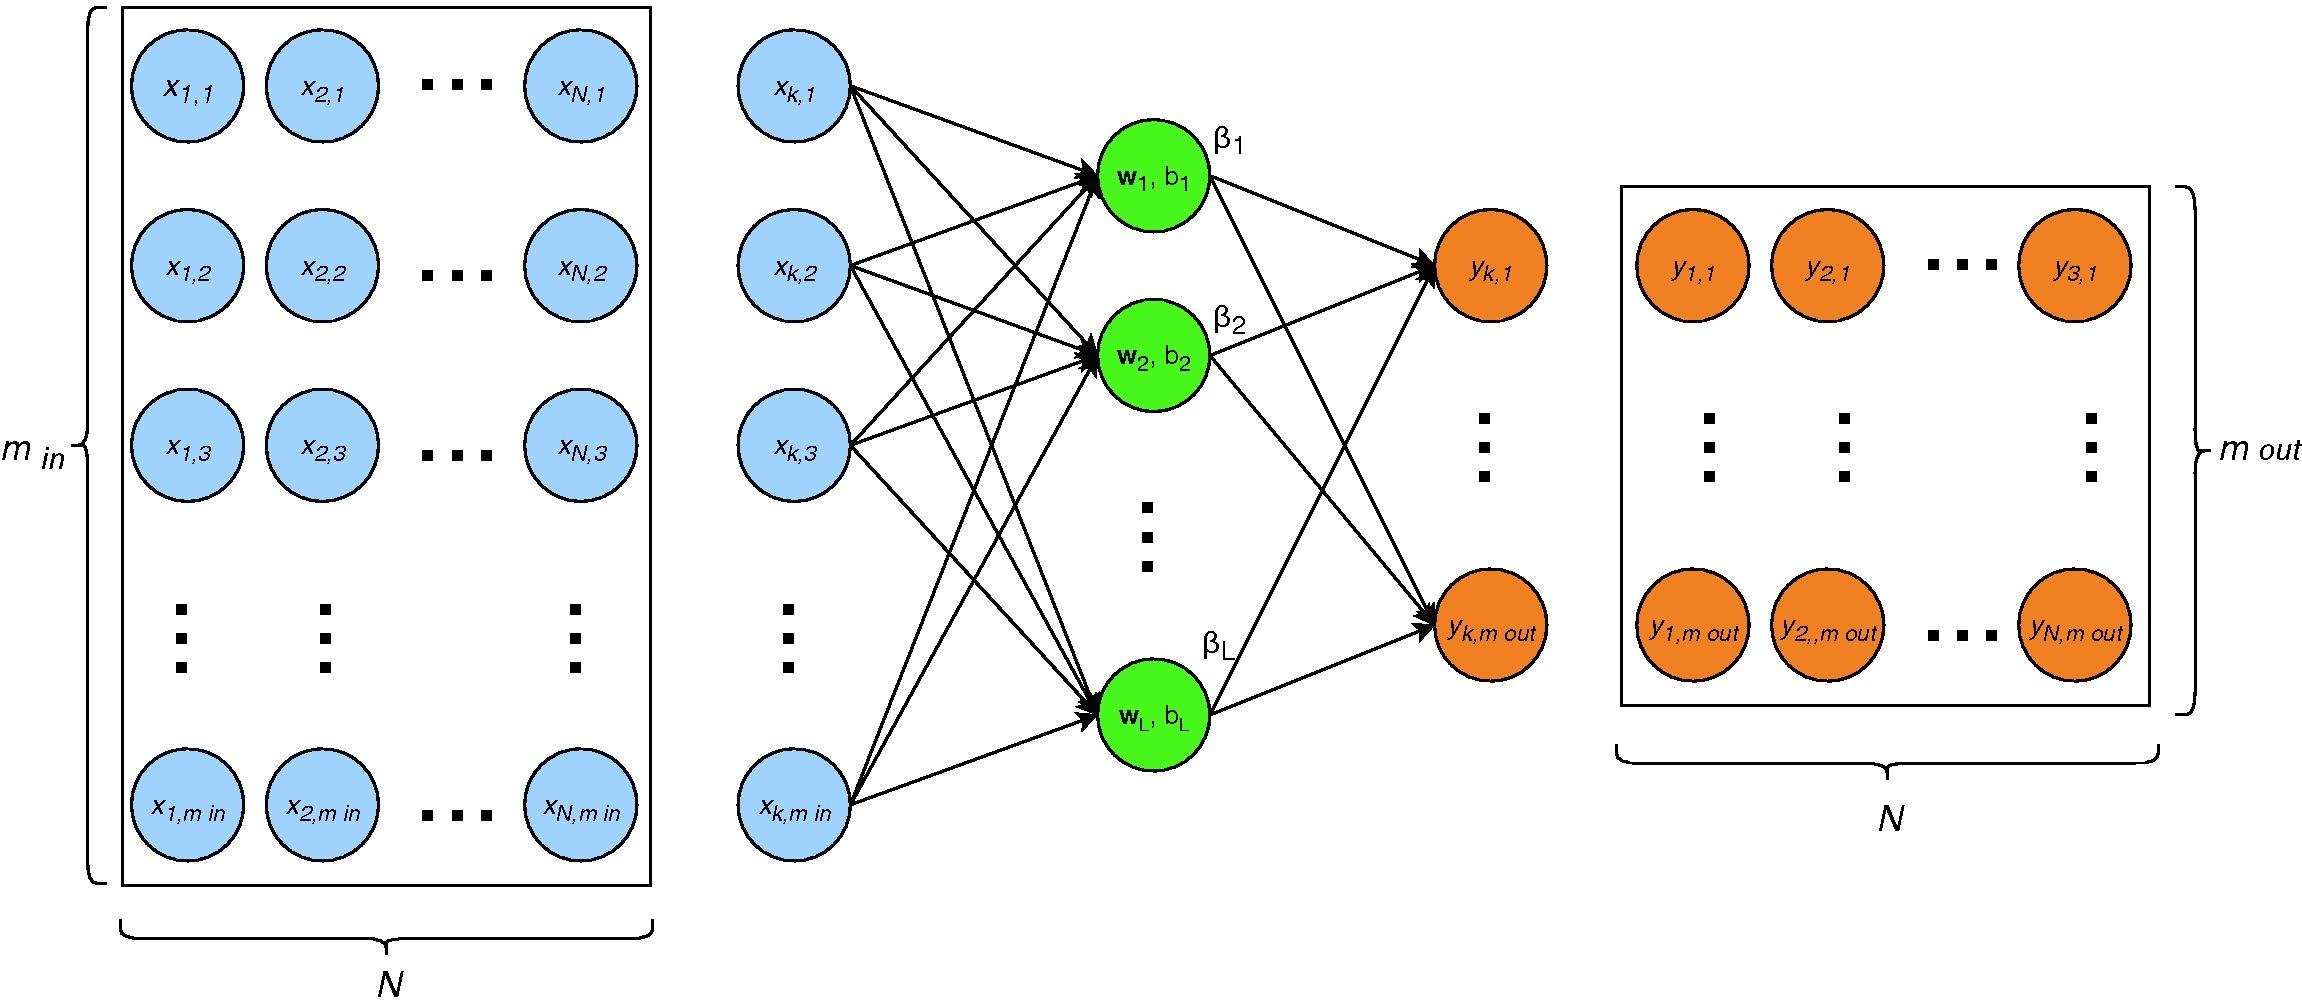
\includegraphics[width=0.8\textwidth]{chapters/tikhonov_s2/images/net}
    \label{fg:1}
\end{figure}
\begin{itemize}
\item Обозначим за $\mathbf{H}$:
\[
\mathbf{H} = 
\begin{bmatrix} 
	h(\mathbf{x}_1,\mathbf{\omega}_1,{b}_1) & \ldots & h(\mathbf{x}_1,\mathbf{\omega}_L,{b}_L)\\
	\vdots & \ddots & \vdots \\
	h(\mathbf{x}_N,\mathbf{\omega}_1,{b}_1) & \ldots & h(\mathbf{x}_N,\mathbf{\omega}_L,{b}_L)\\
\end{bmatrix},
\quad
\mathbf{H} \in \mathbb{R}^{N \times L}
\]

\item Решается задача оптимизации:
\[
   \mathbf{\hat{\beta}} = \arg\min_{\beta}\frac{C}{2}\|\mathbf{H}\beta - \mathbf{T}\|^2 + \frac{1}{2}\|\beta\|^2,
   \quad
   \mathbf{T} = 
    \begin{bmatrix} 
    	\mathbf{t}_1^T\\
    	\vdots \\
    	\mathbf{t}_N^T\\
    \end{bmatrix}
   \quad,
   \mathbf{\beta} = 
    \begin{bmatrix} 
    	\mathbf{\beta}_1^T\\
    	\vdots \\
    	\mathbf{\beta}_L^T\\
    \end{bmatrix},
\]
где $\mathbf{T}$ - вектор истинных ответов, $\mathbf{\beta}$ - вектор весовых коэффициентов, $C$ - масштабирующий коэффициент.
\end{itemize}
В этом случае цель состоит в том, чтобы обучить, как в пакетном, так и в последовательном режиме, SLFN для представления взаимосвязи между положением космического корабля вокруг небольшого интересующего тела и значением гравитационного ускорения.
Работа полагается на серию физических моделей для точного представления пространственного изменения гравитационного поля вокруг небольшого тела и выборки положения космического корабля для создания обучающей выборки.
Впоследствии используется теория ELM, чтобы эффективно обучать сеть изучению желаемых отношений. После обучения и проверки SLFN на основе ELM способен обрабатывать новую входную позицию (то есть местоположения, которые никогда не были замечены сетью) и быстро вычислять соответствующее гравитационное ускорение.
Этот метод особенно подходит для ситуаций, которые требуют быстрых и точных вычислений гравитационного поля как функции положения (например, распространение траекторий космического корабля на борту во время операций вблизи поверхности очень неправильного тела).
В дальнейшем предлагаемый подход оценивается при моделировании гравитационного поля астероида 25143 Итокава и кометы 67P / Чурюмова-Герасименко.

Высокоточные модели многогранников используются для генерации желаемого обучающего набора и для оценки эффективности предложенного подхода к моделированию ELM для определения как локального, так и глобального гравитационного поля.
\begin{figure}[h]
    \centering
    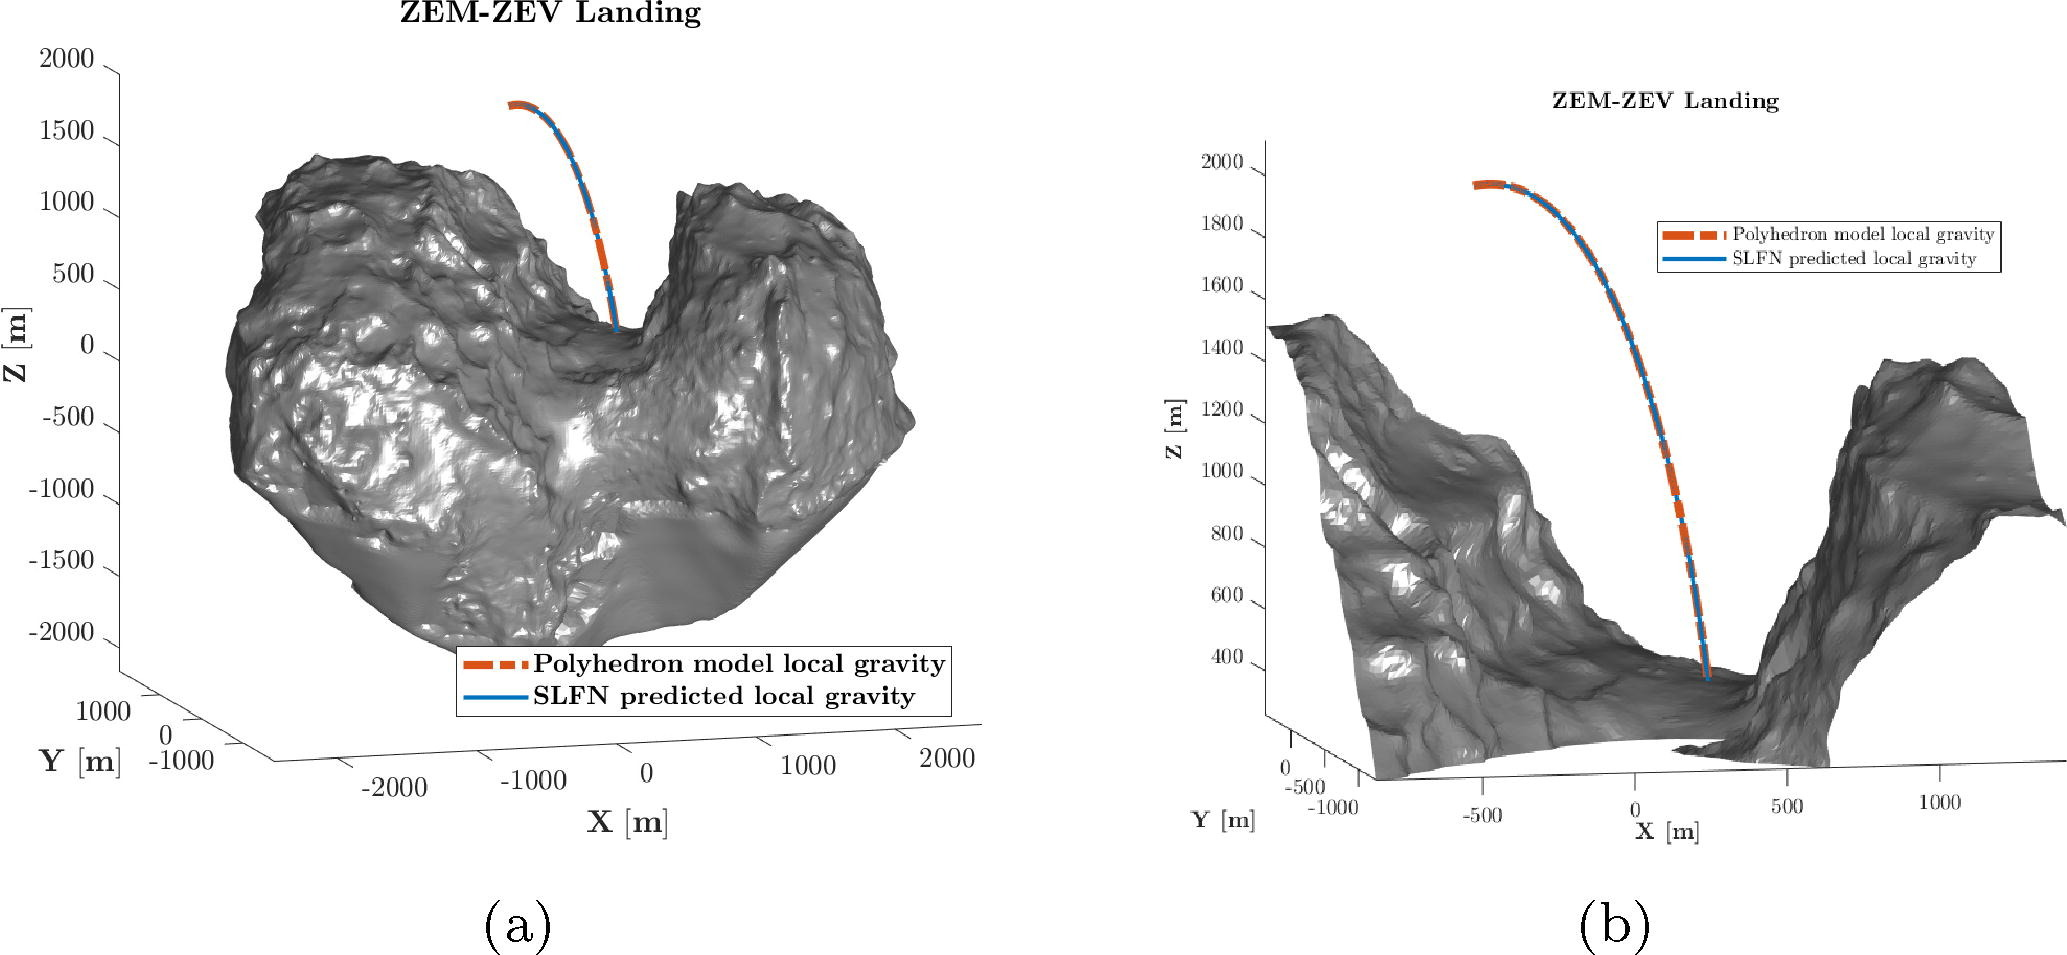
\includegraphics[width=0.8\textwidth]{chapters/tikhonov_s2/images/traj_2}
    \caption{Посадка на комету 67P/Чурюмова-Герасименко: изображение траектории спуска.}
    \label{fg:1}
\end{figure}

Ускорение силы тяжести на основе ELM также используется для вычисления оптимальной по энергии команды ускорения с обратной связью, которая может иметь место во время сценариев управляемой посадки в реальном времени.
\section{Questions To Discussion}
\begin{enumerate}
    \item Какие еще есть варианты решения?
    \item Почему не использовалась простая интерполяция вточках с заранее подсчитанным гравитационным потенциалом?
    \item Чем ELM метод лучше классической МНС?
    \item Почему авторы статьи разделили обучающую выборку на разные сферические области?
\end{enumerate}